40. \begin{figure}[ht!]
\center{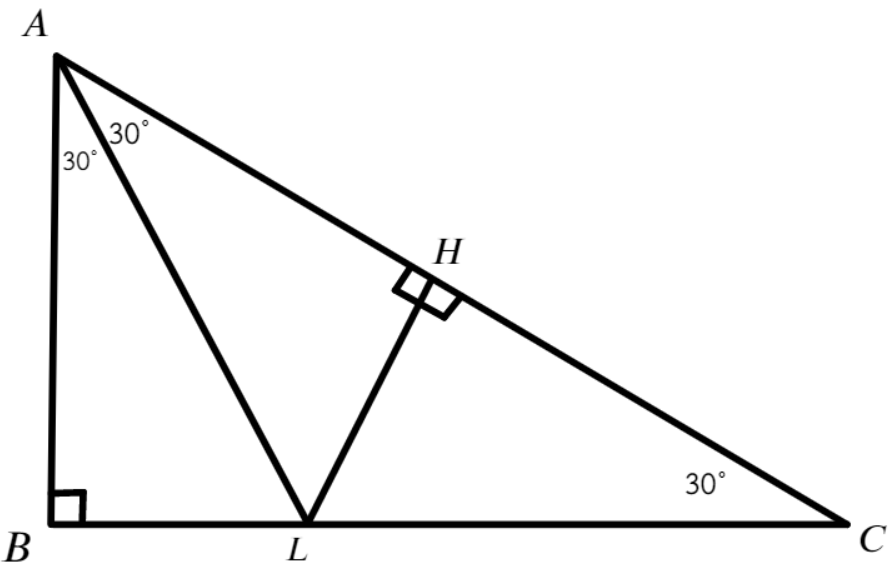
\includegraphics[scale=0.35]{g40.png}}
\end{figure}\\
Угол $B$ равен $180^\circ-90^\circ-60^\circ=30^\circ.$ Так как $AL$ является биссектрисой, $\angle BAL= \angle LAH=60^\circ:2=30^\circ.$ Тогда по теорема о катете, лежащем напротив угла в $30^\circ,$ для треугольников $LCH,\ LAH$ и $ABL$ имеем $AL=LC=2LH,\ BL=\frac{1}{2}AL=LH.$ Тогда $BC=BL+LC=LH+2LH=3LH.$ Таким образом, $LH=BC:3=6:3=2$см.\\
